
\clearpage
\subsection{Validació 2: Càlcul d'isotermes} \label{sec:validacio_02}

Una segona opció de validació del codi és comparar els resultats que aquest proporciona amb una referència fiable. En aquest cas s'ha calculat el mapa de temperatures i les corbes isotermes entre les temperatures de $23 \ \celsius$ i $32 \ \celsius$ pel temps $t = 5000 \ \second$. La discretització espacial emprada ha estat la següent: $N_1 = 90$, $N_2 = 108$, $L_1 = 90$, $L_2 = 70$, $L_3 = 40$. Això dona lloc a una discretització de $40400$ nodes. Per la discretització temporal s'ha escollit un esquema de Crank--Nicolson amb $\Delta t = 0.10 \ \second$. El criteri de convergència per la resolució del sistema d'equacions ha estat $\delta = 10^{-12}$ i $\textsf{itmax} = 500$. El temps de càlcul per aquesta discretització ha estat d'aproximadament $25$ minuts.

En la figura \ref{fig:isotermes} es mostren els resultats obtinguts amb el codi de simulació en \MATLAB i en la figura \ref{fig:isotermes_cttc} els resultats donats per la referència \cite{cttc}.
\vspace*{-0.40cm}
\begin{figure}[h]
	\centering
	\begin{tikzpicture}
		\node[anchor=south west,inner sep=0] at (0,0) {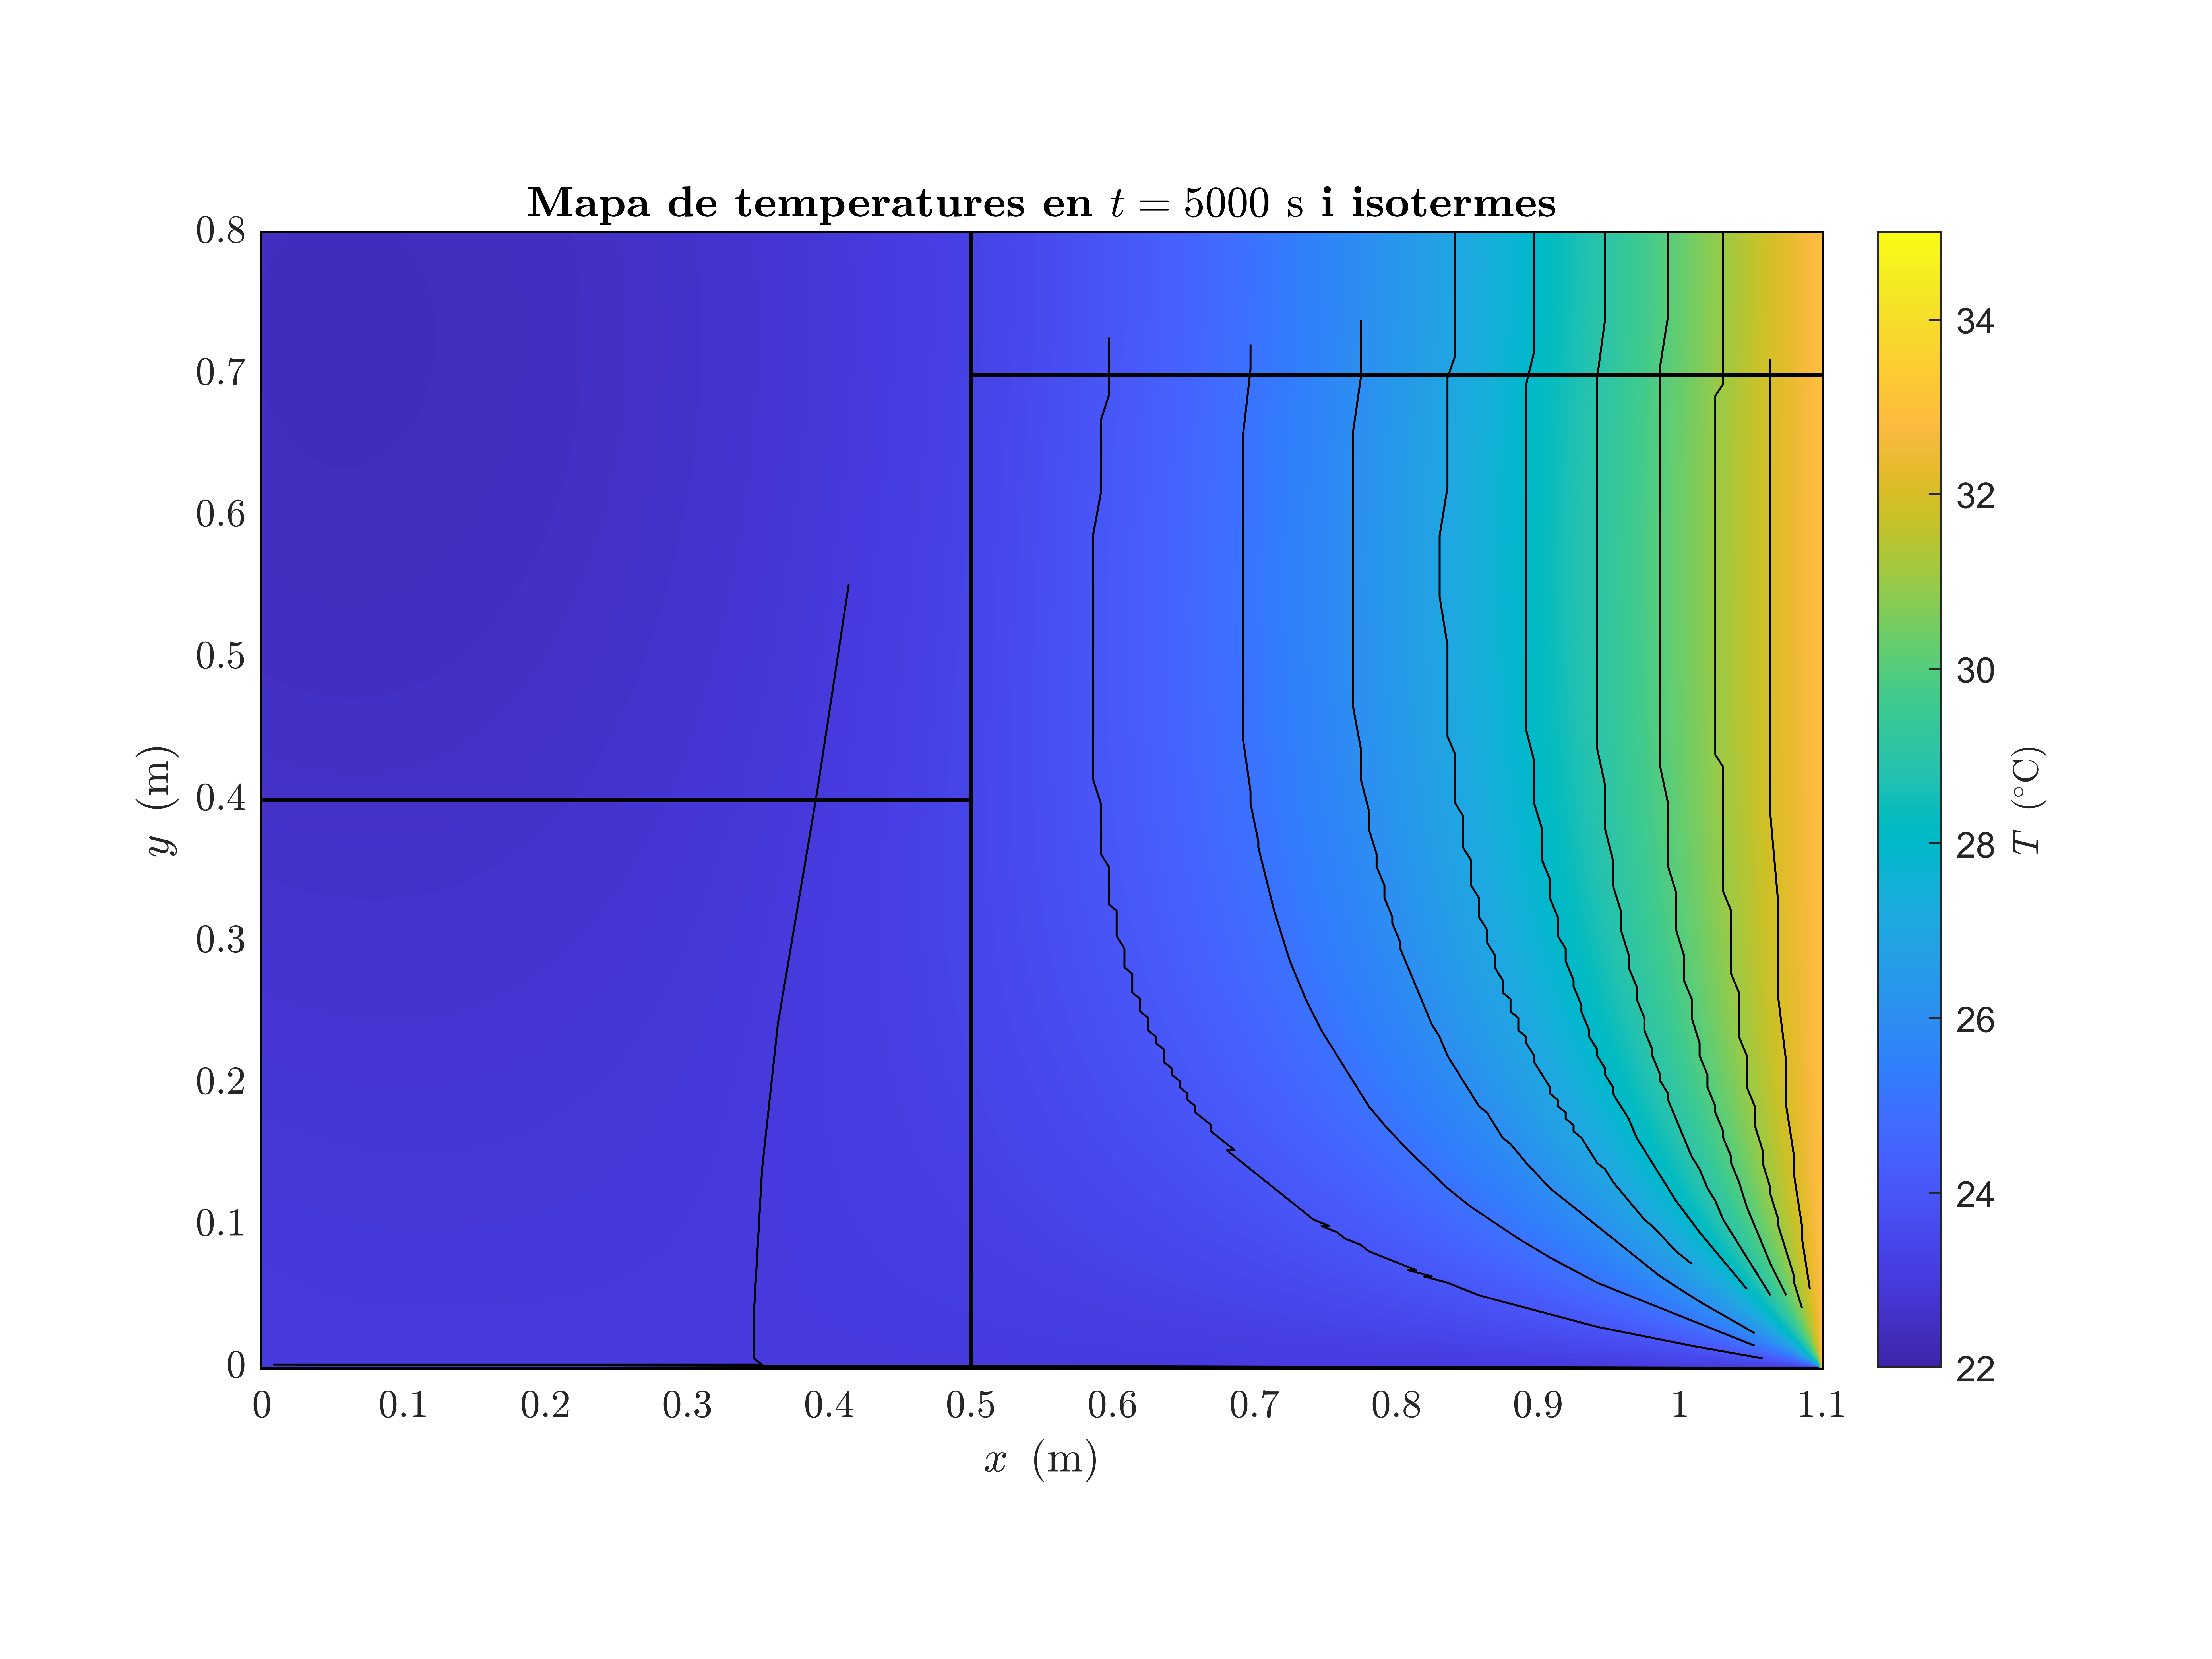
\includegraphics[width=12cm]{imagenes/03_validacio/isotermes.png}};
		\node (rect) at (4.3,4) [draw,thick, rounded corners=.1cm, minimum width=0.3cm, minimum height=0.3cm, fill=black!30!green,rotate=90] {\tiny{$23$}};
		\node (rect) at (6.1,4) [draw,thick, rounded corners=.1cm, minimum width=0.3cm, minimum height=0.3cm, fill=black!30!green,rotate=90] {\tiny{$24$}};
		\node (rect) at (6.9,4) [draw,thick, rounded corners=.1cm, minimum width=0.3cm, minimum height=0.3cm, fill=black!30!green,rotate=90] {\tiny{$25$}};
		\node (rect) at (7.6,4) [draw,thick, rounded corners=.1cm, minimum width=0.3cm, minimum height=0.3cm, fill=black!30!green,rotate=90] {\tiny{$26$}};
		\node (rect) at (7.9,4.6) [draw,thick, rounded corners=.1cm, minimum width=0.3cm, minimum height=0.3cm, fill=black!30!green,rotate=90] {\tiny{$27$}};
		\node (rect) at (8.35,4.6) [draw,thick, rounded corners=.1cm, minimum width=0.3cm, minimum height=0.3cm, fill=black!30!green,rotate=90] {\tiny{$28$}};
		\node (rect) at (8.6,5.2) [draw,thick, rounded corners=.1cm, minimum width=0.3cm, minimum height=0.3cm, fill=black!30!green,rotate=90] {\tiny{$29$}};
		\node (rect) at (9.05,5.2) [draw,thick, rounded corners=.1cm, minimum width=0.3cm, minimum height=0.3cm, fill=black!30!green,rotate=90] {\tiny{$30$}};
		\node (rect) at (9.3,5.8) [draw,thick, rounded corners=.1cm, minimum width=0.3cm, minimum height=0.3cm, fill=black!30!green,rotate=90] {\tiny{$31$}};
		\node (rect) at (9.6,6.4) [draw,thick, rounded corners=.1cm, minimum width=0.3cm, minimum height=0.3cm, fill=black!30!green,rotate=90] {\tiny{$32$}};
	\end{tikzpicture}
	\vspace{-1.2cm}
	\caption{Mapa de temperatures en $t = 5000 \ \second$ i isotermes de $23 \ \celsius$ a $32 \ \celsius$.}
	\label{fig:isotermes}
\end{figure}

\begin{figure}[h]
	\centering
	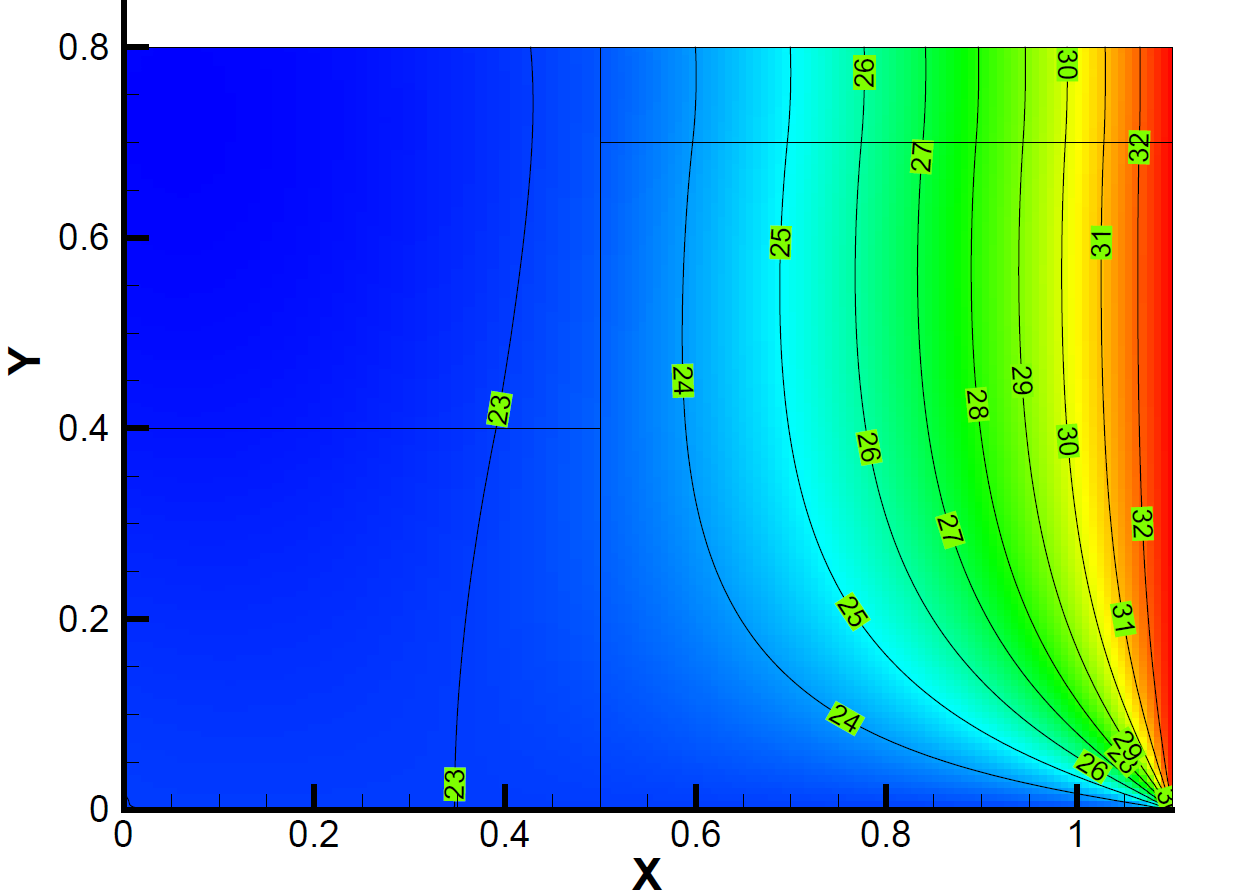
\includegraphics[width=11cm]{imagenes/03_validacio/isotermes_cttc.PNG}
	\caption{Mapa de temperatures en $t = 5000 \ \second$ i isotermes de $23 \ \celsius$ a $32 \ \celsius$ donat per \cite{cttc}.}
	\label{fig:isotermes_cttc}
\end{figure}

S'aprecia que ambdós mapes de temperatura, llevat dels colors escollits, són equivalents. Això indica que els resultats del codi de simulació són fiables. Quant a les isotermes de la figura \ref{fig:isotermes}, s'observa que no recorren tot el domini i que, en general, no són corbes suaus. Una explicació d'aquest fet és la discretització escollida. Escollint una malla més fina, especialment en el material $M_4$, i un pas de temps $\Delta t$ més petit, els resultats seran més precisos i s'aproparan més als donats per \cite{cttc}. Tanmateix, els creixents temps de càlcul són prohibitius, raó per la qual s'han considerat satisfactoris el resultats de la figura \ref{fig:isotermes}.

Dels resultats obtinguts en les dues validacions, es conclou que el codi de simulació de transferència de calor satisfà els principis físics bàsics.



